\documentclass[tikz]{standalone}

\usepackage[latin1]{inputenc}
\usepackage{tikz}
\usetikzlibrary{quotes,angles}
% GNUPL
% Draw line annotation
% Input:
%   #1 Line offset (optional)
%   #2 Line angle
%   #3 Line length
%   #5 Line label
% Example:
%   \lineann[1]{30}{2}{$L_1$}
\newcommand{\lineann}[4][0.5]{%
    \begin{scope}[rotate=#2, blue,inner sep=2pt]
        \draw[densely dashed, blue!40] (0,0) -- +(0,#1)
            node [coordinate, near end] (a) {};
        \draw[densely dashed, blue!40] (#3,0) -- +(0,#1)
            node [coordinate, near end] (b) {};
        \draw[|<->|] (a) -- node[fill=white] {#4} (b);
    \end{scope}
}
\begin{document}
\pagestyle{empty}


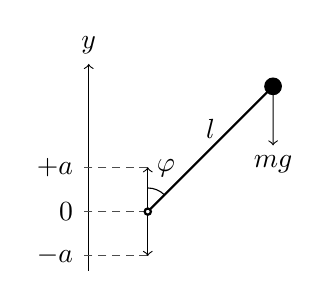
\begin{tikzpicture}[scale=0.75]
    \draw[->] (0,-1) -- (0,2.5) node[above] {$y$};
    % \begin{scope}[xshift=1cm]
        % \lineann[-0.5]{45}{3}{$l$}
    % \end{scope}
    \draw [black!70, densely dashed] (1,0) -- ++(-1.1,0) node [left,black] {$0$};
    \draw [black!70, densely dashed] (1,0.75) -- ++(-1.1,0) node [left,black] {$+a$};
    \draw [black!70, densely dashed] (1,-0.75) -- ++(-1.1,0) node [left,black] {$-a$};
    \draw [<->] (1,-0.75) -- (1,0.75);
    \draw [black, thick] (1,0) -- node[above] {$l$} ++(45:3);
    % \coordinate [label=left:$0$] (0) at (0,0);
    % \coordinate [label=center:$a$] (3) at (0.5,0.25);
    % \coordinate [label=center:$a$] (3) at (0.5,-0.25);
    % \coordinate [label=center:$\varphi$] (3) at (1.2,0.4);
    % \coordinate [label=center:$l$] (3) at (2,1.5);
    % \coordinate [label=center:$mg$] (3) at (3.5,2);
    % \draw[black,thick] (1,0.25) to [out=0,in=90] (1.15,0.18);
    \draw[fill=black] (1,0) coordinate (b) -- ++(45:3) circle (4pt);
    \draw [->] (1,0) -- ++(45:3) coordinate (a) -- ++(0,-1) node[below] {$mg$};
    \coordinate (c) at (1,2);
    \draw pic["$\varphi$", draw=black, -, angle eccentricity=2, angle radius=0.3cm]  {angle=a--b--c};
    \draw[fill=white,thick] (1,0) circle (1.5pt);
\end{tikzpicture}


\end{document}